\chapter{Обзор предметной области}
\section{Технологии, использующиеся в приложении}
	Данный проект, как и другие интернет-приложения,  состоит из клиентской и серверной части. В этой главе даётся краткий обзор тех технологий и языков программирования, которые использовались для написания обоих частей.
\subsection{Клиентская часть}
	Для написания клиентской части используются следующие технологии и языки программирования:
\begin{itemize}
	\item \textbf{HTML/CSS} -- стандартные технологии веб программирования, используемые для верстки веб приложения.
	\item \textbf{JavaScript} -- высокоуровневый динамический язык программирования, который используется в основном для клиентской части интернет-приложений. Позволяет взаимодействовать с пользователем, изменять видимый пользователю документ, отправлять AJAX-запросы серверу. JavaScript позволяет писать как в функциональном, так и в объектно-ориентированном стиле, однако используемое в языке ``прототипное наследование'' обусловливает отличия в работе с объектами по сравнению с традиционными языками, использующими классы.
	\item \textbf{Jquery} -- распространённая библиотека для JavaScript, которая добавляет простой и достаточно удобный интерфейс для отправки запросов к серверу, обработки событий, взаимодействия с DOM-деревом и многого другого.
	\item \textbf{Jquery UI} -- библиотека, основанная на JQuery. Предоставляет интерфейс для создания различных элементов сайта, таких как диалоги, вкладки, кнопки и.т.д.
	\item \textbf{CodeMirror} -- редактор кода, написанный на языке JavaScript. Данный редактор является стандартом де-факто для тех приложений, в которых требуется редактировать/демонстрировать код. На данный момент поддерживает более 100 языков и обладает достаточно простым интерфейсом, позволяющим легко поддержать любой новый язык. Так же он обладает системой плагинов, которая позволяет его персонализировать, добавляя те возможности, которые вас интересуют (например, поиск, автодополнение, подсветка текущей строки и.т.д.)
	\item \textbf{Котлин} -- статически типизированный объектно-ориентированный язык программирования, который может быть скомпилирован в JavaScript. Котлин, как и JavaScript, позволяет писать не только в объектно-ориентированном, но и в функциональном стиле. Так же в Котлине создан ряд абстракций (аннотация native, dynamic тип и др.), которые позволяют взаимодействовать с кодом на JavaScript. Благодаря этому, в большинстве случаев, код, написанный на JavaScript, достаточно легко транслируется в код на Котлине. 
\end{itemize}

\subsection{Сервер}
	Серверная часть приложения написана на языке Java. В качестве сервера используется Tomcat.

	\textbf{Tomcat} -- сервер, написанный на языке Java и разрабатываемый компанией Apache. Tomcat реализует ряд спецификаций языка Java, таких как Java Servlet и JavaServer Pages. Для обработки запросов, приходящих на сервер, томкат использует отдельные потоки, количество которых может регулироваться в настройках сервера. 
	
	Также в серверной части приложения используется \textbf{MySql} -- реляционная база данных.
	
\section{Технологии, использующиеся для тестирования}
	Тестирование интернет-приложения, как правило, состоит из нескольких частей -- тестирования клиентского кода, тестирование серверного кода, а так же тестирование поведения сервера при большом количестве запросов (нагрузочное тестирование).
	
	Для проведения этих частей тестирования в данном проекте используются следующие технологии:
	\begin{itemize}
\item Тестирование серверного кода:
	\begin{itemize}
		\item \textbf{JUnit} -- распространённая библиотека для написания unit-тестов на языке Java.
	\end{itemize}
\item Нагрузочное тестирование:
	\begin{itemize}
		\item \textbf{JMeter} -- графическое Java приложение, предназначенное для написания нагрузочного тестирования и измерения производительности при нагрузочном тестировании. Данное приложение позволяет отправлять различного рода запросы (нас интересуют HTTP запросы) и анализировать производительность сервера при обработке этих запросов.
	\end{itemize}
\item Тестирование клиентского кода:
\begin{itemize}
	\item \textbf{nodejs} -- платформа, позволяющая запускать код на языке JavaScript. Обычно используется для создания серверов и сетевых приложений. В данном проекте используется для запуска karma.
	\item \textbf{karma} -- приложение для запуска тестов на языке JavaScript. Может исполнять тесты во всех популярных браузерах(Google Chrome, Opera, Safari \dots), а так же внутри phantomjs. Это приложение само написано на JavaScript и предназначено для запуска при помощи nodejs.
	\item \textbf{phantomjs} -- браузер без графического интерфейса, созданный для автоматического тестирования веб приложений. Данный браузер основан на платформе WebKit, что делает его похожим по поведению на такие браузеры как Chrome и Safari.
	\item \textbf{qunit} -- распространённая библиотека для написания unit-тестов на языке JavaScript.
\end{itemize}
\end{itemize}

\section{Публикация интернет-приложений}
В данной главе освещаются технологии, используемые нами для публикации приложения.
\subsection{Amazon Web Services}
	Amazon Web Service -- это набор сервисов, предоставляемый компанией Amazon. Данные сервисы предоставляют возможность создания масштабируемой инфраструктуры на машинном уровне и состоят из следущих компонент:
\begin{itemize}
	\item \textbf{Amazon EC2 instance} -- пожалуй, один из основных элементов всей инфраструктуры. EC2 instance -- это компьютер, предоставляемый амазоном, параметры которого можно выбирать при старте, основываясь на требованиях к данному компьютеру. В зависимости от параметров меняется и стоимость данного компьютера.
	\item \textbf{Amazon Machine Image (AMI)} -- снимок памяти компьютера, необходим для того, чтобы запустить EC2 instance. Существует большое количество публичных AMI, которые, как правило, содержат операционную систему (например, для запуска EC2 instance с Ubuntu необходимо найти идентификатор AMI содержащего Ubuntu  и указать его при старте машины). Так же пользователь может создать свой AMI, содержащий специфичную для данной задачи информацию.
	\item \textbf{Launch Configuration} -- конфигурация, которая содержит все данные, необходимые для запуска EC2 instance, такие как: 
	\begin{itemize}
		\item Instance type -- определяет мощность CPU, количество памяти и другие подобные параметры  EC2 instance.
		\item AMI ID -- идентификатор AMI
		\item User Data -- скрипт, который будет исполнен после запуска машины. Позволяет автоматизировать запуск машины.
		\item ...
	\end{itemize}
	\item \textbf{Cloud Watch Monitoring} -- сервис, который собирает и хранит информацию о других сервисах, например, для каждого EC2 instance хранятся: 
	\begin{itemize}
		\item Потребление CPU
		\item Количество операций чтения/записи на диск
		\item \dots
	\end{itemize}
	Вся эта информация доступна через веб интерфейс Amazon. %ссылка на какую-нибудь картинку%.
	\item \textbf{Cloud Watch Monitoring Alarm} -- настраиваемые события внутри Cloud Watch Monitoring. Например, ``среднее потребление CPU у EC2 instnance более 80\% в течении 5 минут''. Может использоваться как для оповещения администратора, так и для управления масштабированием
	\item \textbf{Auto Scaling Group (ASG)} -- система, позволяющая запускать заданное количество EC2 instance. Их количество может выставляться как вручную, так и на основании Cloud Watch Monitoring Alarmsdamnaleto-ов.
	\item \textbf{Elastic Load Balancer (ELB)} -- балансировщик нагрузки. Распределяет приходящие на него HTTP-запросы между компьютерами, которые к нему подключены.
\end{itemize}


Кроме перечисленных выше сервисов нами использовались сервисы, связанные с безопасностью, доменными именами и.т.д., однако они являются техническими и их описание не представляет особого интереса.

\subsection{Cхема работы автоматического масштабирования в AWS}
	Перечисленные выше сервисы, как правило, не используются сами по себе, а собираются в большую систему. В данном параграфе я покажу как в общем из описанных выше сервисов получается автоматически масштабируемая система.
	
	Схема работы автоматического масштабирования приведена на рис.\ref{fig:aws_autoscaling}.
	
\begin{figure}[h]
    \centering
    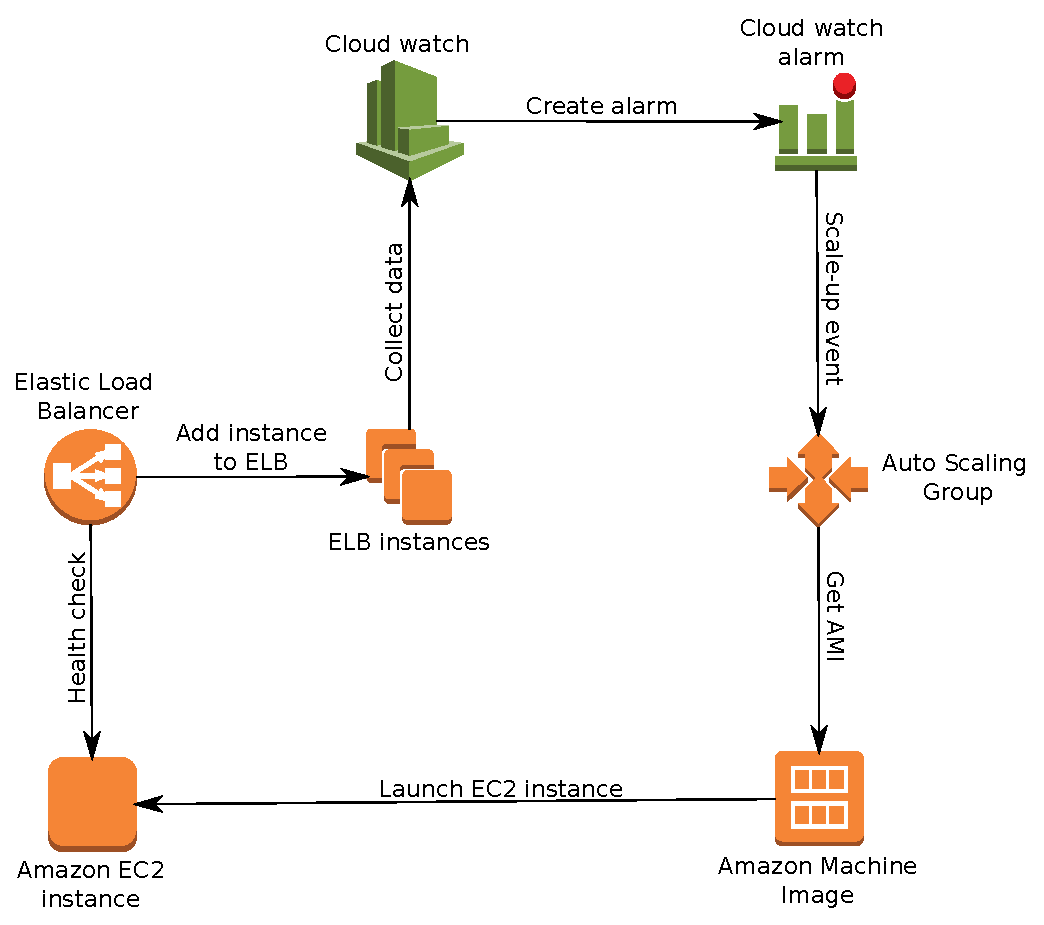
\includegraphics[scale=0.8]{amazon_scale_up.eps} 
    \caption{Принципиальная схема работы автоматического масштабирования в AWS}
    \label{fig:aws_autoscaling}
\end{figure}
	Рассмотрим как это всё работает начиная с процесса создания. Первым создаётся балансировщик нагрузки (ELB). В начале к нему не прикреплен ни один компьютер, поэтому, если на него приходит запрос, то он просто отвечает HTTP статусом 503 (сервис недоступен).
	
	Далее создаётся система автоматического масштабирования (ASG). При её создании необходимо иметь конфигурацию (Launch Configuration), основываясь на которой она будет запускать новые компьютеры в случае надобности. Также нужно создать события (Cloud Watch Alarms), которые будут послать сигналы для увеличения/уменьшения количества машин в системе масштабирования. Каждое из этих событий следит за потреблением одного из ресурсов, например, потреблением CPU и позволяет отреагировать на то, что мы данный ресурс исчерпываем (нужно запустить больше машин), либо у нас его слишком много (нужно остановить несколько машин).
	
	После создания система, используя заданную конфигурацию, автоматически поднимает минимальное количество машин (параметр, передающийся при запуске) и подключает их к ELB. Балансировщик нагрузки выполняет проверку того, что переданные ему машины работоспособны (определённым образом отвечают на определённый запрос) и, как только убеждается в их работоспособности, начинает отправлять туда запросы.
	
	Дальнейшее масштабирование происходит на основе данных в системе мониторинга (Cloud Watch Monitoring). Данные, полученные с запущенных машин, сравниваются с настроенными нами событиями и на основании их система масштабирования автоматически  запускает (аналогично предыдущему пункту), либо останавливает компьютеры.
	
	Кроме описанного выше случая компьютер может быть остановлен если он в какой-то момент не пройдёт проверку работоспособности от ELB. В такой ситуации система масштабирования попытается поднять новую машину на замену неработоспособной. Это позволяет автоматически восстанавливать систему если что-то произошло на одном из компьютеров, однако может привести к неприятным последствиям, которые будут освещены в главе \ref{}.

\subsection{Docker}

	Docker - технология виртуализации, которая последнее время набирает всё большую популярность среди разработчиков. 
	
	Отличие докера от виртуальных машин, которые также являются способом виртуализации, заключается в основном в легковесности. Каждая виртуальная машина должна кроме приложения (которое может иметь размер в несколько мегабайт) подгружать ещё и окружение (которое может иметь размер в несколько гигабайт). В отличии от этого докер-контейнер содержит только приложение и его зависимости и запускается в изолированном процессе в пространстве пользователя, разделяя ядро с другими контейнерами.
\begin{figure}[h]
	\centering
	\begin{subfigure}[b]{.5\textwidth}
  		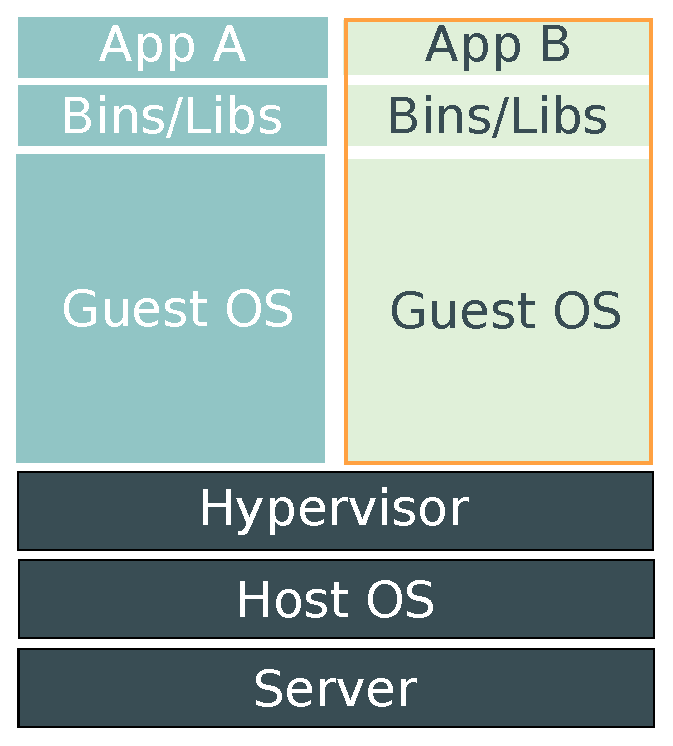
\includegraphics[width=.9\linewidth]{vm_scheme}
  		\caption{Virtual Machines}
  		\label{fig:sub1}
	\end{subfigure}%
	\begin{subfigure}[b]{.5\textwidth}
  		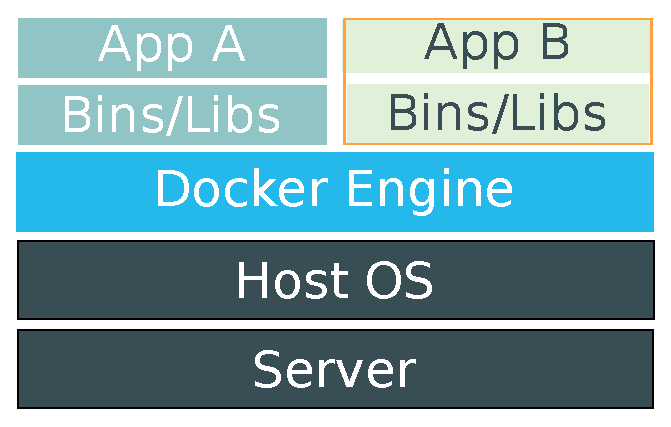
\includegraphics[width=.9\linewidth]{docker_scheme}
  		\caption{Docker}
  		\label{fig:sub2}
	\end{subfigure}
	\caption{Сравнение виртуализации при помощи виртуальных машин и при помощи докер контейнеров}
	\label{fig:test}
\end{figure}

	Каждый докер-контейнер основан докер-образе. Докер-образ это шаблон, по которому мы можем запускать контейнеры. В нём мы можем указать операционную систему, которую мы хотим использовать, установить необходимое окружение, и.т.д. Образы можно как собирать, основываясь на файле с инструкциями, так и скачивать с хранилищ.
	
	Каждый образ состоит из слоёв. Слой это состояние контейнера после того, как мы выполнили очередную команду. Такая структура позволяет нам при обновлениях образа вместо обновления всего приложения обновить только изменившиеся слои.
\subsection{Операционная система}
\begin{itemize}

	\item {\bf CoreOS} - операционная система, предназначенная для запуска всего внутри контейнеров Linux, например, при помощи докера, о котором шла речь в предыдущем пункте. В связи с такой специфической направленностью в CoreOS отсутствуют почти все привычные для пользователя Linux пакеты и программы (yum, apt-get, wget \dots), грубо говоря, там есть только докер.
	
	\item {\bf systemd} - демон инициализации других демонов в Linux. Systemd позволяет описывать сервис, который мы собираемся запустить, в текстовом виде. Ниже приведён пример файла сервиса, который запускает докер контейнер.
\begin{lstlisting}
[Unit]
Description=My Service
Requires=docker.service
After=docker.service

[Service]	
ExecStart=/usr/bin/docker run busybox /bin/sh -c "while true; do echo Hello World; sleep 1; done"

[Install]
WantedBy=multi-user.target
\end{lstlisting}
\end{itemize}
	Кроме запуска systemd следит за работоспособностью запущенных сервисов и, если какой-то из них возвращает ошибку, перезапускает его (если не настроить обратное).
\section{Обновление приложений}
Существует множество различных способов обновления интернет-приложения в зависимости от требований к нему. Самыми простыми из них являются:
\begin{itemize}
	\item {\bf Выключать приложение для обновления.} Данный подход является наиболее простым, однако обладает рядом очевидных недостатков, а именно:
	\begin{itemize}
		\item Приложение недоступно в течении обновления.
		\item Невозможно протестировать обновлённое приложение перед его публикацией.
		\item Сложно восстановить работоспособность приложения при неудачном обновлении.
	\end{itemize}
	\item {\bf Создавать копию приложения вместе с инфраструктурой.} При таком подходе обновляется то приложение, которое на данный момент не принимает запросы от пользователя. После обновления все запросы начинают отправляться на новую версию приложения, а старая версия становится неактивной до следующего обновления. Недостатком такого подхода является необходимость создания копии всей инфраструктуры.
	\item {\bf Создавать копию приложения (Blue-Green deployment).} Данный подход известен  как аналогичен предыдущему, но в нём неактивное приложение располагается внутри той же инфраструктуры, что и активное. Недостатки данного подхода будут описаны подробней в главе \ref{sec}
\end{itemize}